\documentclass{beamer}
\usepackage[russian]{babel}
\usetheme{metropolis}

\usepackage{adjustbox}
\usepackage{makecell}

\usepackage{amsthm}
\setbeamertemplate{theorems}[numbered]

\setbeamercolor{block title}{use=structure,fg=white,bg=gray!75!black}
\setbeamercolor{block body}{use=structure,fg=black,bg=gray!20!white}

\usepackage[T2A]{fontenc}
\usepackage[utf8]{inputenc}

\usepackage{hyphenat}
\usepackage{amsmath}
\usepackage{graphicx}

\AtBeginEnvironment{proof}{\renewcommand{\qedsymbol}{}}{}{}

\title{
Микроэкономика-I
}
\author{
Павел Андреянов, PhD
}

\begin{document}

\maketitle

%\section{План}
%
%\begin{frame}{План}
%
%В первой половине лекции мы рассмотрим две важные темы: налогообложение, и  понятия чистых субститутов и комплементов.
%
%Во второй половине лекции мы поговорим о компенсирующих вариациях и Матрицах Слуцкого.
%
%\end{frame}


%\section{Напомним себе}
%
%\begin{frame}{Напомним себе}
%
%\begin{table}[hbt]
%\centering
%\begin{adjustbox}{width=1\textwidth}
%  \begin{tabular}{l|c|c|c|c|}
%    & КД-1 & КД-2 & Леонтьев & Линейная \\
%    \hline
%    $U$ & $\alpha \log x + \beta \log y$ & $x^{\alpha} y^{\beta}$ & $\min(x/a, y/b)$ & $x/a + y/b$ \\
%    \hline
%    $m_x$ & $\frac{\alpha}{\alpha + \beta} \frac{I}{p}$ & ... & $\frac{ap}{ap+bq}\frac{I}{p}$ & $\frac{I}{p}$ или $0$ \\
%    \hline
%    $V$ & \makecell[l]{$(\alpha + \beta)\log I - $\\ $- \alpha \log p - ...$} & $\frac{I^{\alpha + \beta}}{p^{\alpha} q^{\beta}} \cdot K_1$ & $\frac{I}{ap + bq}$& $\frac{I}{\min(ap,bq)}$ \\
%    \hline
%    $E$ & $(\frac{p^{\alpha} q^{\beta}}{K_1} 
%    log \bar U)^{\frac{1}{\alpha + \beta}}$ & $(\frac{p^{\alpha} q^{\beta}}{K_1} \bar U)^{\frac{1}{\alpha + \beta}}$ & $(ap+bq) \cdot \bar U$ & $\min(ap,bq) \cdot \bar U$\\
%    \hline
%    $h_x$ & $\frac{\alpha}{\alpha + \beta} p^{\frac{-\beta}{\alpha + \beta}} \cdot K_2$ & ... & $a \cdot \bar U$ & $a \cdot \bar U$ или $0$\\
%    \hline
%  \end{tabular}
%  \end{adjustbox}
%\end{table}
%Kонстанты $K_1, K_2$ вычислите сами.
%
%
%\end{frame}
%
%\section{Больше задач}
%
%\begin{frame}{Задача 1}
%
%Петя на завтрак ест омлет и $x_1$ яиц и $x_2$ стаканов молока, и испытывает полезность $$ U_{om}(x_1,x_2) = \log x_1 + 3 \log x_2$$  
%а также салат из $y_1$ помидоров из $y_2$ моцареллы $$ U_{salad}(y_1,y_2) = \min(y_1,y_2).$$
%Омлет и салат являются совершенными субститутами.
%$$ U(\vec x, \vec y) = U_{om}(\vec x) + U_{salad}(\vec y).$$
%Посчитайте в каком соотношении Петя разделит 1000 руб. между двумя блюдами, если цены товаров равны 1,2,3,4 руб.
%
%\end{frame}
%
%\begin{frame}{Задача 2}
%
%Петя на завтрак ест омлет и $x_1$ яиц и $x_2$ стаканов молока, и испытывает полезность $$ U_{om}(x_1,x_2) = x_1/2 + x_2/3$$  
%а также салат из $y_1$ помидоров из $y_2$ моцареллы $$ U_{salad}(y_1,y_2) = \sqrt{y_1 y_2}.$$
%Омлет и салат являются совершенными комплементами.
%$$ U(\vec x, \vec y) = \min(U_{om}(\vec x),U_{salad}(\vec y)).$$
%Посчитайте в каком соотношении Петя разделит 1000 руб. между двумя блюдами, если цены товаров равны 1,2,3,4 руб.
%
%\end{frame}
%
%\section{Больше задач}
%
%\begin{frame}{Задача 3}
%
%Петя ест на завтрак бутерброд из черной икры $x$ и хлеба $y$:
%$$ U_{bb}(x,y) = \log x + 2 \log y$$
%Цену хлеба нормируем к 1 а цена черной икры пусть равна $p$. Всего у Пети есть 1000 рублей, но запрещено покупать более 1 банки черной икры (на руки).
%
%\end{frame}
%
%\begin{frame}{Задача 3}
%
%\begin{itemize}
%  \item Сформулируйте задачу максимизации полезности
%  \item Является ли она выпуклой
%  \item Выпишите УПП
%  \item При каких ценах решение внутреннее?
%  \item Выпишите ответ.
%\end{itemize}
%
%\end{frame}
%
%\begin{frame}{Задача 4}
%
%Петя ест на завтрак бутерброд из черной икры $x$ и хлеба $y$:
%$$ U_{bb}(x,y) = \min(x, 2y)$$
%Цену хлеба нормируем к 1 а цена одной банки черной икры пусть равна $p$. Всего у Пети есть 1000 рублей, но запрещено покупать более 1 банки черной икры (на руки). Однако, можно (до-)купить икру на черном рынке по удвоенной цене $2p$.
%\end{frame}
%
%\begin{frame}{Задача 4}
%
%\begin{itemize}
%  \item Сформулируйте задачу максимизации полезности
%  \item Является ли она выпуклой
%  \item Выпишите необходимые условия (УПП или их аналог)
%  \item Пойдет ли Петя на черный рынок?
%  \item Выпишите ответ.
%\end{itemize}
%
%\end{frame}
%
%\section{Налоги}
%
%\begin{frame}{Налоги}
%
%Исторически сложилось так, что государство финансирует свою деятельность, а также производство общественных благ за счет налогообложения. Есть три вида налогов:
%
%\begin{itemize}
%\item \alert{подоходный фиксированный}, или паушальный (от нем. "Pauschale"), налог
%\item \alert{подоходный пропорциональный} налог
%\item \alert{товарный} налог
%
%\end{itemize}
%
%В разные периоды времени разные налоги пользовались популярностью. 
%
%\end{frame}
%
%\begin{frame}{Паушальный налог}
%
%Простота паушального налога в том, что его можно ввести практически моментально, и его имплементация сводится к знанию своих подданных в лицо. Однако вы не можете установить паушальный налог больше, чем, грубо говоря, минимальный прожиточный минимум. 
%
%То есть, чтобы собрать большую сумму паушальным налогом, вам придется освободить какую-то часть населения от этих налогов. Как только вы начинаете дискриминировать, то есть говорить кому платить, а кому не платить налог, он становится в какой-то степени пропорциональным.
%
%\end{frame}
%
%\begin{frame}{Пропорциональный налог}
%
%Обычный пропорциональный налог означает, что каждый агент платит пропорционально своему доходу. К примеру, когда король Ричард Львиное Сердце попал в плен, английской короне пришлось платить выкуп за счет временного пропорционального налогообложения размером 25\%. 
%
%Таким образом, удалось в короткие сроки собрать огромную по тем временам сумму, примерно составляющую трехгодовой объем английской казны.
%
%\end{frame}
%
%\begin{frame}{Подоходные налоги}
%
%\begin{figure}[hbt]
%\centering
%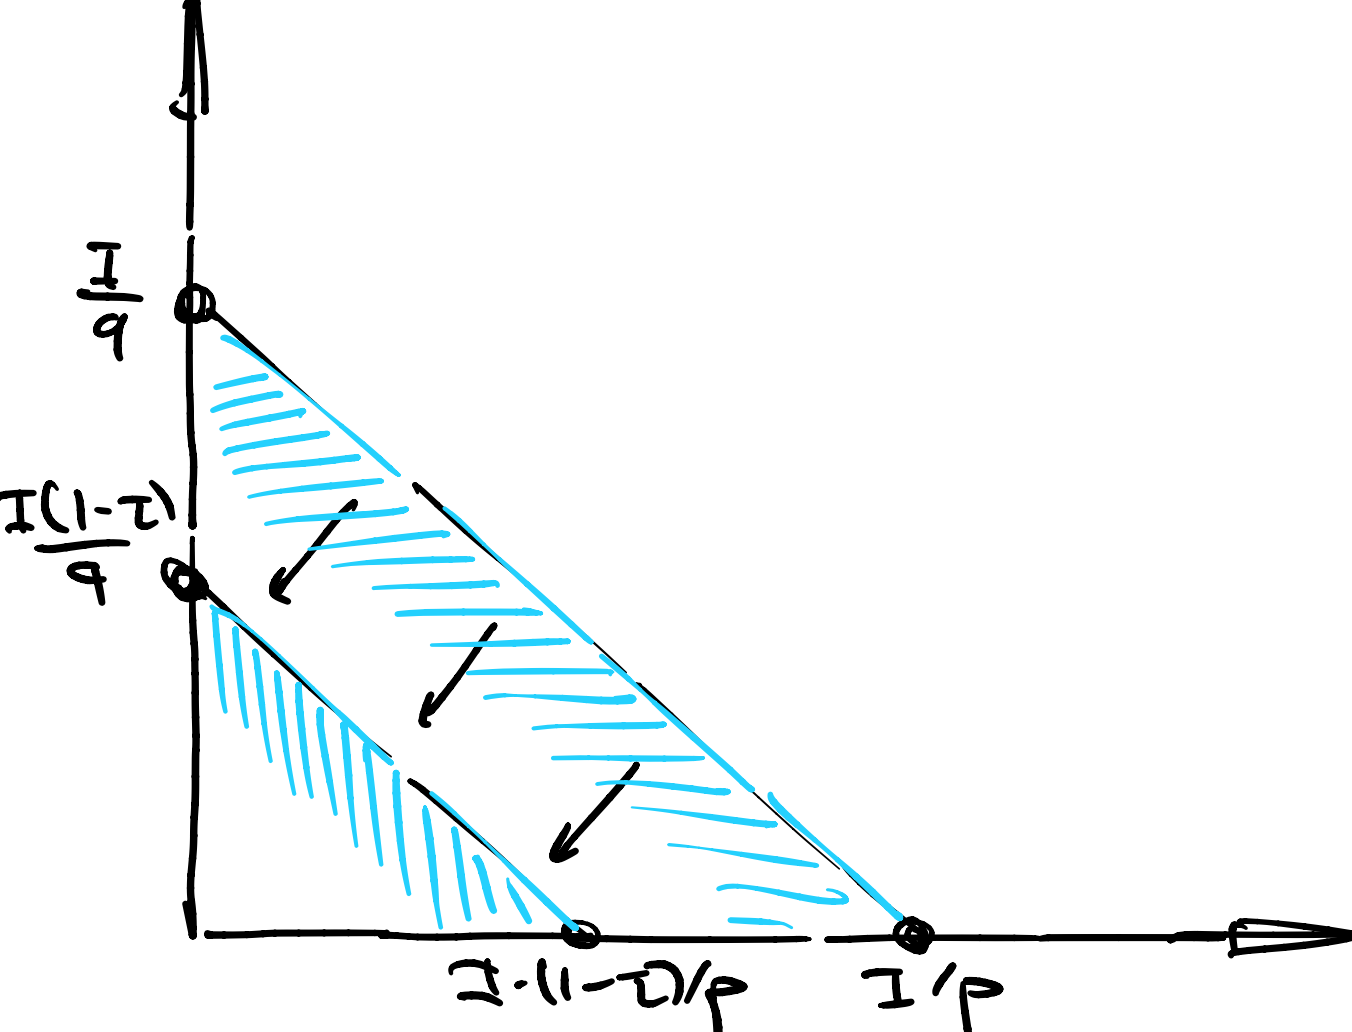
\includegraphics[width=.8 \textwidth]{podohod_nalog.png}
%\end{figure}
%
%\end{frame}
%
%\begin{frame}{Товарный налог}
%
%Товарный налог хорошо адаптируется под быстро меняющуюся экономику. Например, если какой-то город начинает экономически расти, растут требования к окружающей его инфраструктуре: дороги, дома для рабочих, школы и университеты и так далее. Но также растут продажи товаров и услуг и, соответственно, растут налоговые сборы, покрывающие инвестиции в инфраструктуру.
%
%\end{frame}
%
%\begin{frame}{Товарный налог}
%
%\begin{figure}[hbt]
%\centering
%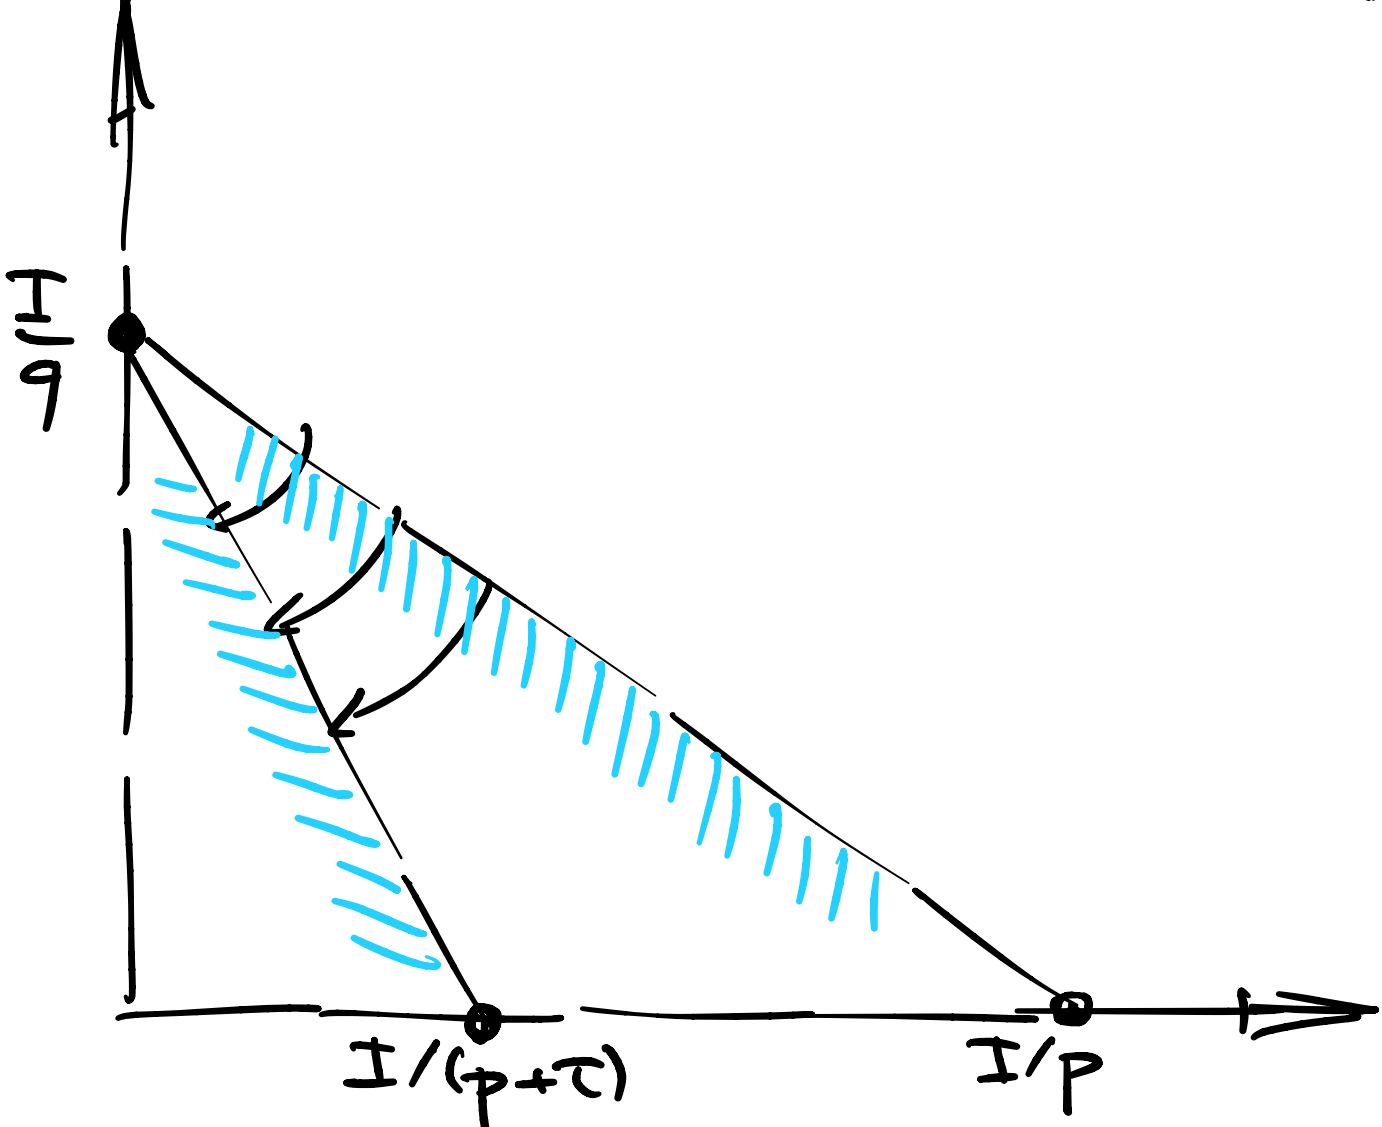
\includegraphics[width=.8 \textwidth]{tovarny_nalog.png}
%\end{figure}
%
%\end{frame}
%
%\begin{frame}{Налоги}
%
%Задача налогообложения может быть сформулирована как либо максимизация чистых налоговых сборов, либо максимизация косвенной полезности при фиксированных налоговых сборах. 
%
%На выбор есть подоходный и товарный налог.
%
%\end{frame}
%
%\section{Налоги в Коббе-Дугласе}
%
%\begin{frame}{Кобб-Дуглас}
%
%Рассмотрим полезность Кобба-Дугласа 
%$$U(x,y) = \alpha \log x + \beta \log y$$
%
%и введем налог размера $\tau$. Наш анализ оптимального налогообложения будет сильно зависеть от того, с какой легкостью мы выписываем косвенную полезность.
%
%\end{frame}
%
%\begin{frame}{Кобб-Дуглас}
%
%Если налог подоходный (доля $\tau$), то налоговые сборы будут равны $T = \tau I$ а косвенная полезность:
%$$ V(p,q,I|\tau) = (\alpha + \beta)\log I + \log (1-\tau) - \alpha \log(p) - \beta \log (q) + C$$
%Максимизация чистых налоговых своров тут не представляет сложности - надо просто выставить $\tau = 1$, то есть отобрать все деньги. 
%
%Максимизация косвенной полезности при фиксированных налоговых сборах тоже тривиальна: $\tau = T/I$.
%
%\end{frame}
%
%\begin{frame}{Кобб-Дуглас}
%
%Пусть товарные налоги равны $\tau_x, \tau_y$ соответственно, тогда косвенная полезность равна:
%$$V(p,q,I|\tau_x, \tau_y) = (\alpha + \beta)\log I - \alpha \log(p + \tau_x) - \beta \log (q + \tau_y) + C$$
%а налоговые сборы:
%$$T = \frac{\alpha}{\alpha + \beta} \frac{I}{p+\tau_x}\tau_x + \frac{\beta}{\alpha + \beta} \frac{I}{q+\tau_y} \tau_y$$
%
%\end{frame}
%
%\begin{frame}{Кобб-Дуглас}
%
%Максимизация чистых налоговых сборов – это задача безусловной оптимизации:
%$$T =  \frac{\alpha}{\alpha + \beta} I \frac{\tau_x}{p+\tau_x} + \frac{\beta}{\alpha + \beta} I \frac{\tau_y}{q+\tau_y}$$
%
%У этой задачи смешное решение: необходимо назначить бесконечно большой налог на оба товара, тогда удастся собрать, в пределе, точно $I$. 
%
%Это не очень реалистично.
%
%\end{frame}
%
%\begin{frame}{Кобб-Дуглас}
%
%Максимизация косвенной полезности при фиксированных налоговых сборах – это задача условной оптимизации. 
%
%Она уже более интересная:
%$$- \alpha \log(p + \tau_x) - \beta \log (q + \tau_y) \to \max$$
%При ограничении $$\alpha \frac{\tau_x}{p+\tau_x} + \beta \frac{\tau_y}{q+\tau_y} \geqslant (\alpha + \beta)\frac{T}{I}$$
%или
%$$\alpha \frac{-p}{p+\tau_x} + \beta \frac{-q}{q+\tau_y} \geqslant (\alpha + \beta)(\frac{T}{I}-1)$$
%
%Является ли эта задача выпуклой?
%
%\end{frame}
%
%\begin{frame}{Кобб Дуглас}
%
%$$ \mathcal{L} = - \alpha \log(p + \tau_x) - \beta \log (q + \tau_y) + \lambda (\alpha \frac{-p}{p+\tau_x} + \beta \frac{-q}{q+\tau_y})$$
%
%Условия первого порядка по $\tau_x$, $\tau_y$:
%$$ - \frac{\alpha}{p + \tau_x} + \lambda \frac{\alpha p}{(p + \tau_x)^2} = 0, \quad - \frac{\beta}{q + \tau_y} + \lambda \frac{\beta q}{(q + \tau_y)^2} = 0$$
%
%Другими словами,
%$$\frac{p + \tau_x}{p} = \lambda = \frac{q + \tau_y}{q}$$
%
%То есть кажется, что оптимальные налоги должны быть выставлены пропорционально ценам (это же НДС!!!). 
%
%\end{frame}
%
%\begin{frame}{Кобб Дуглас}
%
%Нам очень повезло, и Гессиан, действительно, отрицательно определен:
%$$ \frac{\partial^2 \mathcal{L}}{\partial^2 \tau_x} = \frac{-\alpha}{(p+\tau_x)^2}, \quad \frac{\partial^2 \mathcal{L}}{\partial^2 \tau_y} = \frac{-\beta}{(p+\tau_y)^2}$$
%
%Значит наше внутреннее решение - локальный оптимум.
%
%\end{frame}
%
%\begin{frame}{Кобб Дуглас}
%
%Складывается впечатление, что оптимальные налоги в Кобб-Дугласе устроены так, что они не меняют доли расходов, потраченные на каждый товар. Более того, если присмотреться, то этот налог эквивалентен подоходному налогу, ведь он тоже не меняет доли. 
%
%Другими словами, когда товарные налоги пропорциональны ценам в Кобб-Дугласе, то бюджетное множество сдвигается параллельно, в точности как у подоходного налога.
%
%\end{frame}
%
%\begin{frame}{Кобб Дуглас}
%
%Мы только что доказали, хоть и в малой общности, оптимальность единого НДС.
%
%\begin{lemma}[Оптимальность НДС]
%Оптимальный налог в Кобб-Дугласе это единый НДС.
%\end{lemma}
%
%\end{frame}
%
%\section{Правило Рамсея}
%
%\begin{frame}{Фрэнк Рамсей}
%\begin{columns}
%\begin{column}{0.5\textwidth}
%   \alert{Фрэнк Рамсей} (Frank Plumpton Ramsey) британский математик и экономист начала 20 века. Своей целью он ставил \alert{минимизировать ненужные потери общества} при потреблении путём введения \alert{дифференцированной ставки налогообложения} на различные товары. 
%\end{column}
%\begin{column}{0.5\textwidth}  %%<--- here
%    \begin{center}
%     \includegraphics[width=1\textwidth]{ramsay}
%     \end{center}
%\end{column}
%\end{columns}
%\end{frame}
%
%\begin{frame}{Правило Рамсея}
%
%Это в точности максимизация косвенной полезности при зафиксированных налоговых сборах:
%\begin{gather*}
%\mathcal{L} = V(p+\tau_x,q+\tau_y) \\ - \lambda (\tau_x m_x(p+ \tau_x,q+\tau_y) + \tau_y m_y(p+ \tau_x,q+\tau_y) - T)
%\end{gather*}
%Выпишем условия первого порядка (по $\tau_x, \tau_y$):
%$$\frac{\partial V}{\partial p} = \lambda [\tau_x \frac{\partial m_x}{\partial p} + m_x], \quad \frac{\partial V}{\partial q} = \lambda [\tau_y \frac{\partial m_y}{\partial q}+m_y]$$
%Вспомним тождество Роя:
%$$-\frac{\partial V}{\partial I}m_x = \lambda [\tau_x \frac{\partial m_x}{\partial p}+m_x], \quad -\frac{\partial V}{\partial I}m_y = \lambda [\tau_y \frac{\partial m_y}{\partial q}+m_y]$$
%\end{frame}
%
%\begin{frame}{Правило Рамсея}
%
%несколько хитрых операций с дробями и получим
%$$ \frac{m_x}{m_y} = \frac{\tau_x \frac{\partial m_x}{\partial p} + m_x}{\tau_y \frac{\partial m_y}{\partial q}+m_y} \quad \Leftrightarrow \quad \frac{m_x \frac{\partial m_y}{\partial q}}{m_y \frac{\partial m_x}{\partial p}} = \frac{\tau_x}{\tau_y}$$
%Мы только что доказали (немножко игнорируя вопросы выпуклости) один из самых нетривиальных фактов в теории оптимального налогообложения, называемое Правилом Рамсея.
%
%\end{frame}
%
%\begin{frame}{Правило Рамсея}
%
%То же самое правило можно получить если минимизировать функцию расходов агента вместо максимизации его полезности:
%\begin{gather*}
%\mathcal{L} = E(p+ \tau_x,q+\tau_y) + \\ + \lambda (\tau_x h_x(p+ \tau_x,q+\tau_y) + \tau_y h_y(p+ \tau_x,q+\tau_y))
%\end{gather*}
%Выпишем условия первого порядка (по $\tau_x, \tau_y$) вспоминая по ходу Лемму Шепарда (i.e., Теорему об Огибающей):
%$$h_x = \frac{\partial E}{\partial p} = \lambda [\tau_x \frac{\partial h_x}{\partial p}+h_x], \quad h_y = \frac{\partial E}{\partial q} = \lambda [\tau_y \frac{\partial h_y}{\partial q}+h_y]$$
%
%\end{frame}
%
%\begin{frame}{Правило Рамсея}
%
%\begin{lemma}
%Оптимальные налоговые ставки (в процентах) обратно пропорциональны эластичностям (маршаллианского в основной задаче и хиксианского в двойственной) спроса:
%$$ \frac{\tau_x/p}{\tau_y/q} = \frac{-1/\varepsilon_{x,p}}{-1/\varepsilon_{y,q}},$$
%\end{lemma}
%другими словами, менее эластичные товары должны облагаться более сильным налогом, чем более эластичные.
%
%Прямо как в задаче монополиста.
%
%\end{frame}
%
%\section{Чистые субституты и комплементы}
%
%\begin{frame}{Чистые субституты и комплементы}
%
%Напомню, что первое определение субститутов и комплементов опиралось на перекрестные производные (маршаллианских) спросов по ценам. 
%
%Несмотря на кажущуюся простоту и интуитивность этого определения, ничего не сдерживало нас от построения таких примеров, где товар $х$ был бы субститутом к $y$, при этом $y$ был комплементом к $x$.
%
%Сейчас мы дадим альтернативное определение субститутов и комплементов. Для экспозиции предположим два товара $х,y$ с ценами $p,q$.
%\end{frame}
%
%\begin{frame}{Чистые субституты и комплементы}
%
%\begin{definition}
%\alert{Чистыми субститутами} называются пары товаров:
%$$
%\frac{\partial h_x}{\partial q} > 0, \quad \frac{\partial h_y}{\partial p} > 0.
%$$
%
%\alert{Чистыми комплементами} называются пары товаров: 
%$$
%\frac{\partial h_x}{\partial q} \leqslant 0, \quad \frac{\partial h_y}{\partial p} \leqslant 0.
%$$
%\end{definition}
%
%\end{frame}
%
%\begin{frame}{Чистые субституты и комплементы}
%
%На первый взгляд, не совсем понятно, чем помогает замена Маршалианского спроса на Хиксианский в определении. Однако, поскольку Хиксианский спрос – это градиент функции расходов, градиент Хиксианского спроса – это Гессиан функции расходов. 
%
%А Гессиан, он же матрица Гессa - симметричная матрица.
%
%\end{frame}
%
%\begin{frame}{Чистые субституты и комплементы}
%
%\begin{lemma}
%Пусть $h$ - весь вектор Хиксианского спроса, тогда
%$$ \nabla \vec h = \nabla^2 E \quad \Rightarrow \quad \nabla \vec h = (\nabla \vec h)^T.$$
%\end{lemma}
%
%Другими словами, перекрестные производные Хиксианского спроса по ценам - симметричны и нет больше никакого противоречия. Чистая субститутабильность и комплементарность – это свойство пары товаров, неважно как эта пара упорядочена.
%
%Попробуем ответить на вопрос (на доске) являются ли товары попарно чистыми субститутами в моделях Кобб-Дугласа, Леонтьева и линейной полезности.
%
%\end{frame}
%
%\section{Перерыв}

\begin{frame}{Налоги и компенсации}

Мы освоили технику оптимального налогообложения. Это очень удобно, но иногда все равно приходится идти на попятную и точечно корректировать доход отдельным людям, возможно, из социально незащищенных слоев населения.

Поставим задачу вычисления денежной компенсации, которая сбалансирует экзогенное повышение цен, связанное с \alert{налогами} или \alert{санкциями}.

\end{frame}

\section{Наивная компенсация}

\begin{frame}{Наивная компенсация}

Сфокусируемся на одном товаре пока.

Предположим, что полезность агентов была изначально на уровне $\bar U_0$ и произошло смещение цен $p \to p+\Delta p$. Как правило, нас интересует именно повышение цен. Пусть потребление товара при цене $p$ было на уровне $x = x_0$.

Например, из за санкций повысились цены на оригинальные кофейные картриджи nespresso, на запчасти автомобилей...

Полезность агентов, конечно же, упала на новый уровень $\bar U_1$.

\end{frame}

\begin{frame}{Наивная компенсация}

Итак, цены, потребление и полезность изменились $$p, x_0, \bar U_0 \to p + \Delta p, x_1, \bar U_1$$
Если у вас совсем мало времени, то можно предложить наивную компенсацию агенту в размере $$\Delta W_{naive} = \Delta p \cdot x_0$$ то есть, в точности разницу в расходах из за санкций.

Вопрос: \alert{Значит, полезность агент останется такой же?}

\end{frame}

\begin{frame}{Наивная компенсация}

На самом деле, нет, полезность агента вырастет. Убедимся
$$ U = \log x + \log y, \quad W = 8$$
Пусть цены выросли от $(1,1)$ до $(2,1)$, тогда потребление изменилось от $(4,4)$ до $(2,4)$. 

Наивная компенсация равна в точности
$$ \Delta W_{naive} = (2-1) \cdot 4 = 4$$
Однако, при суммарном бюджете в $W=12$ агент будет потреблять $(3,6)$ а вовсе не $(4,4)$. 

Убедимся что полезность его вырастет: $$ \log 18 =\log 3 + \log 6 > 2 \log 4 = \log 16$$

\alert{Почему?}

\end{frame}

\begin{frame}{Наивная компенсация}

Из за замещения потребления в результате смещения цен, наивная компенсация получилась слишком большой.

Как бы нам сделать эту компенсацию поменьше.

\end{frame}

\section{Компенсирующая вариация}

\begin{frame}{Компенсирующая вариация}
Определим компенсирующую вариацию как надбавку к доходу, которая вернет полезность на старый уровень $\bar U_0$, подразумевая что цены так и останутся на завышенном уровне.

\begin{definition} \alert{Компенсирующая вариация} определяется как изменение в расходах, ассоциированных со старым уровнем полезности
$$CV = \Delta W_{comp} := E(p+ \Delta p,\bar U_0) - E(p,\bar U_0)$$
где $U_0$ это старое значение полезности $V(p, W)$.
\end{definition}

Другими словами, государство как бы говорит: "извините, мы вам все возместим, мы вам \alert{компенсируем} за повышение цен".

\end{frame}

\begin{frame}{Компенсирующая вариация}
Альтернативное определение компенсирующей вариации это решение нелинейного уравнения 
$$ V(p+\Delta p,W + \Delta W) = V(p, W)$$
Я утверждаю, что оба метода дают одинаковое $\Delta W_{comp}$. 

Убедимся на доске для кобб дугласа, для которого мы уже знаем все формулы
$$ V(p,q,W) = (\alpha + \beta) \log W - \alpha \log p - \beta \log q + K$$
$$ E(p,q,\bar U) = \exp[\frac{\bar U - K + \alpha \log p + \beta \log q}{\alpha + \beta}]$$

\end{frame}

\begin{frame}{Компенсирующая вариация}

Любопытно, что будет если разложить компенсирующуп вариацию в ряд Тэйлора в окрестности $\Delta p =0$.
$$CV = E(p+ \Delta p,\bar U_0) - E(p,\bar U_0) \approx \nabla E(p,\bar U_0) \cdot \Delta p$$
А чему равна $\nabla E$?

\end{frame}

\begin{frame}{Компенсирующая вариация}

Правильно, $\nabla E$ равна спросу (хиксианскому) при старом уровне полезности, то есть, то что мы называли $x_0$.
$$CV \approx x_0 \cdot \Delta p$$
Получается, что $\Delta W_{naive}$ это просто линейный член в разложении в ряд $\Delta W_{comp}$ (он же  $CV$).

\end{frame}

\section{Эквивалентная вариация}

\begin{frame}{Эквивалентная вариация}

Предположим, что опять смещение цен $p \to p'$ и что полезность агентов упала до уровня $\bar U_1$. Однако, в этот раз пусть это будет обратимое действие. 

Например, в Думу было предложено равномерно увеличить налог НДС. Союз пенсионеров рассчитывает <<дать взятку>>, чтобы заблокировать этот проект.

Чему равен максимальный размер такой <<взятки>>?

\end{frame}

\begin{frame}{Эквивалентная вариация}

Определим эквивалентную вариацию как уменьшение дохода, которая оставит полезность на новом измененном уровене $\bar U_1$, подразумевая что цены откатятся назад.

\begin{definition}

\alert{Эквивалентная вариация} определяется как изменение в расходах, ассоциированных с новым уровнем полезности
$$EV = \Delta W_{equi} := E(p+ \Delta p,\bar U_1) - E(p,\bar U_1)$$
где $\bar U_1 = V(p+\Delta p, W)$.
\end{definition}
Другими словами, государство как бы говорит: "сколько ты готов заплатить чтобы вернуть назад, однако для тебя это \alert{эквивалентно} тому что уже есть".

\end{frame}

\begin{frame}{Эквивалентная вариация}
Альтернативное определение эквивалентной вариации это решение нелинейного уравнения 
$$ V(p+\Delta p,W) = V(p, W - \Delta W)$$
Я утверждаю, что оба метода дают одинаковое $\Delta W_{equi}$. 

Убедимся на доске для кобб дугласа, для которого мы уже знаем все формулы
$$ V(p,q,W) = (\alpha + \beta) \log W - \alpha \log p - \beta \log q + K$$
$$ E(p,q,\bar U) = \exp[\frac{\bar U - K + \alpha \log p + \beta \log q}{\alpha + \beta}]$$

\end{frame}

\section{Какой способ лучше?}

\begin{frame}{Медленный подсчет вариаций через $E$}

К примеру, в Леонтьевской полезности $\min(x/a,y/b)$ функция расходов выписывается быстро, если вспомнить, что левый и правый аргумент функции минимума обязаны давать одно и то же значение в оптимуме: 
$$h_x = a \bar U, \quad h_y = b \bar U, \quad E = (pa + qb) \bar U$$
\end{frame}

\begin{frame}{Медленный подсчет вариаций через $E$}

Далее, если цены перешли $(p,q) \to (p',q')$, то полезность перешла 
$$ \bar U_0 = \frac{W}{pa + qb} \quad \to \quad \bar U_1 = \frac{W}{p'a + q'b} $$

Получается, что
\begin{gather*}
CV = (a \Delta p + b \Delta q) \frac{W}{pa + qb}\\
EV = (a \Delta p + b \Delta q) \frac{W}{p' a + q' b}.
\end{gather*}
Вот и все.
\end{frame}

\begin{frame}{Быстрый подсчет вариаций через $V$}

CV и EV  – это решения нелинейных уравнений:
\begin{gather*}
V(p,q,W) = \bar U_0 = V(p',q',W+CV)\\\
V(p,q,W-EV) = \bar U_1 = V(p',q',W)
\end{gather*}
Преимущество этого подхода в том, что сами уровни полезности вам считать не надо, можно сэкономить на выкладках. К тому же, аддитивные и мультипликативные константы (не зависящие от цен) быстро сокращаются.

\end{frame}

\begin{frame}{Быстрый подсчет вариаций через $V$}

Компенсирующая вариация в КД:
\begin{gather*}
 (\alpha + \beta)\log W - \alpha \log p - \beta \log q = \\
 = (\alpha + \beta)\log (W+CV) - \alpha \log p' - \beta \log q'
\end{gather*}
Получается
$$(\alpha + \beta)\log(\frac{W+CV}{W}) = \alpha \log (\frac{p'}{p}) + \beta \log (\frac{q'}{q})$$
Такое уже совсем просто решить.
\end{frame}

\begin{frame}{Быстрый подсчет вариаций через $V$}
Эквивалентная вариация в КД:
\begin{gather*}
 (\alpha + \beta)\log (W - EV) - \alpha \log p - \beta \log q = \\ =
  (\alpha + \beta)\log W - \alpha \log p' - \beta \log q'
\end{gather*}
Получается
$$-(\alpha + \beta)\log(\frac{I - EV}{I}) = \alpha \log (\frac{p'}{p}) + \beta \log (\frac{q'}{q}) $$
Такое уже совсем просто решить.
\end{frame}

\section{Какая $\Delta W$ меньше?}

\begin{frame}{Какая $\Delta W$ меньше?}
Это сложный вопрос, но короткий ответ на него: 
$$\Delta W_{equi} < \Delta W_{comp} < \Delta W_{naiv}$$ в тех ситуациях когда цены растут.

Легко видеть, например, что для косвенных полезностей линейных по доходу функции расхода линейны по уровню полезности. А значит, та вариация которая соответствует <<худшей>> полезности будет меньшей.
\end{frame}

\section{Что еще можно сделать?}

\begin{frame}{Что еще можно сделать?}
Если у вас времени чуть больше, но все же не настолько много чтобы откалибровать полезность целиком, можно разложить CV в ряд до второго члена.
$$CV \approx \nabla E \cdot \delta p + \nabla^2 E \cdot \frac{(\delta p)^2}{2}  < CV$$

Она будет чуть меньше чем просто линейный кусок, потому что $\nabla^2 E$ отрицательно определена, потому что $E$ вогнута как нижняя огибающая линейного (по ценам) семейства.

\end{frame}

\begin{frame}{Что еще можно сделать?}
В частности, если меняется только одна цена $p$ у товара $x$ то
$$CV \approx h_x \cdot \delta p + \frac{\partial h_x}{\partial p} \cdot \frac{(\delta p)^2}{2}$$
и можно вывести элегантную формулу
$$\frac{CV}{W} \approx \frac{p h_x}{W} \cdot (\delta p / p) + \frac{\partial h_x}{\partial p}\frac{p}{h_x} \frac{p h_x}{W}\cdot \frac{(\delta p/p)^2}{2}$$
позволяющую быстро в уме считать компенсирующие вариации, в процентах от дохода, зная одни лишь только доли расходов и эластичности хиксианские

\end{frame}

\begin{frame}{Что еще можно сделать?}

Вот эта формула
$$\frac{CV}{W} \approx s_x \cdot (\delta p / p) + s_x \cdot \varepsilon^h_{x,p} \cdot \frac{(\delta p/p)^2}{2}$$

Представим себе такую ситуацию...
\end{frame}

\begin{frame}{Что еще можно сделать?}

Сидит Мишустин на докладе и его спрашивает президент: \alert{Господин Мишустин, сколько надо компенсировать нашим дорогим пенсионерам за $50\%$ повышение цены на яйца и хлеб?}

Покрываясь потом, Мишустин начинает считать в уме...

\end{frame}

\begin{frame}{Что еще можно сделать?}
Мишустин знает что доля расходов на такие продукты это примерно $25\%$ (то есть, $\frac{1}{4}$) следовательно короткий ответ это доля на процентное изменение цены или $\frac{1}{4} \cdot \frac{1}{2}$ или $12.5$ процентов. 

Мишустин отвечает: 

\alert{Двенадцать с половиной процентов, господин Президент!}

Президент неодобрительно хмурит брови...

\end{frame}

\begin{frame}{Что еще можно сделать?}

Немножко подумав, Мишустин вспомнил хиксианскую эластичность спроса на еду (скажем, -1/2) он быстро корректирует свой ответ вниз на долю умножить на эластичность умножить на квадрат изменения цены пополам или $\frac{1}{4} \cdot \frac{1}{2} \cdot (\frac{1}{2})^2/2 = \frac{1}{2^6}$ или примерно $1.6$ процентов.

Мишустин отвечает: 

\alert{Поправка, одиннадцать процентов, господин Президент!}

Президент расслабляет брови и говорит: 

\alert{Так то лучше, Мишустин.}

\end{frame}

%\section{Первое приближение}
%
%\begin{frame}{Первое приближение}
%
%Посмотрим внимательно на компенсирующую вариацию:
%$$\log(1 + \frac{CV}{I}) = \frac{\alpha}{\alpha + \beta} \log (1 + \frac{\delta p}{p}) + \frac{\beta}{\alpha + \beta} \log (1 + \frac{\delta q}{q})$$
%
%Разлагая в ряд Тейлора получаем
%
%$$\frac{CV}{I} \approx \frac{\alpha}{\alpha + \beta} \frac{\delta p}{p} + \frac{\beta}{\alpha + \beta} \frac{\delta q}{q}$$
%
%Это читается так: если цена $p$ выросла на $X \%$ а цена $q$ выросла на $Y \%$ то компенсирующая вариация должна увеличить бюджет на $\frac{\alpha}{\alpha + \beta} X + \frac{\beta}{\alpha + \beta} Y$ процентов, в первом приближении.
%
%\end{frame}
%
%\begin{frame}{Первое приближение}
%
%Посмотрим еще раз
%$$\frac{CV}{I} \approx \frac{\alpha}{\alpha + \beta} \frac{\delta p}{p} + \frac{\beta}{\alpha + \beta} \frac{\delta q}{q}$$
%Заметим, что 
%$$CV \approx m_x(p,q) \delta p + m_y(p,q) \delta q.$$
%То есть, чтобы сосчитать компенсирующую вариацию в первом приближении, мы просто берем старый уровень потребления и смотрим на приращение расходов.
%
%\end{frame}
%
%\begin{frame}{Первое приближение}
%
%Это не случайность. Дело в том, что мы могли бы разложить в ряд Тейлора CV сразу по определению...
%$$ CV = E(\vec p +  \delta \vec p, \bar U) - E(\vec p, \bar U)$$ 
%... и в матричной форме, тогда
%$$ CV \approx \nabla E \cdot  \delta \vec p$$ 
%a что такое $\nabla E$???
%\end{frame}
%
%\begin{frame}{Первое приближение}
%Это не случайность. Дело в том, что мы могли бы разложить в ряд Тейлора CV сразу по определению...
%$$ CV = E(\vec p +  \delta \vec p, \bar U) - E(\vec p, \bar U)$$ 
%... и в матричной форме, тогда
%$$ CV \approx \nabla E \cdot  \delta \vec p = \vec h \cdot  \delta \vec p, \quad \frac{CV}{I} \approx \vec s \cdot \frac{\delta \vec p}{p}$$ 
%a что такое $\nabla E$??? Это же Хиксианский спрос! 
%
%То есть, процентное увеличение цен надо взвесить пропорционально долям ($\vec s$ - share) товаров в расходах, и это будет приближенно CV, в процентах.
%\end{frame}
%
%\section{Второе приближение}
%
%\begin{frame}{Второе приближение}
%
%Зафиксируем $q$, и пусть меняется только цена $p$.
%
%Определим $\delta p = p'-p$ как приращение цены. Мы хотим приблизить нелинейное уравнение
%$$\log(1 + \frac{CV}{I}) = \frac{\alpha}{\alpha + \beta} \log (1 + \frac{\delta p}{p})$$
%
%подставим все в экспоненту
%$$1 + \frac{CV}{I} = (1 + \frac{\delta p}{p})^{\frac{\alpha}{\alpha + \beta}}$$
%\end{frame}
%
%\begin{frame}{Второе приближение}
%
%разложим в ряд Тейлора до второго члена
%$$1 + \frac{CV}{I} = 1 + \frac{\alpha}{\alpha + \beta} \frac{\delta p}{p} - \frac{1}{2}\frac{\alpha \beta}{(\alpha + \beta)^2} (\frac{\delta p}{p})^2 + \ldots$$
%
%То есть, $CV$ во втором приближении чуть меньше чем в первом
%$$\frac{CV}{I} = s_x (\frac{\delta p}{p}) - \frac{1}{2}\frac{\alpha \beta}{(\alpha + \beta)^2} (\frac{\delta p}{p})^2.$$
%Это происходит из за того, что люди не стоят как вкопанные со своими спросами, а замещают подорожавшие товары на другие, похожие.
%
%А что если несколько цен меняются одновременно?
%\end{frame}
%
%\begin{frame}{Второе приближение}
%Почему бы не разложить в ряд Тейлора CV до 2 порядка?
%$$ CV = E(\vec p +  \delta \vec p, \bar U) - E(\vec p, \bar U)$$ 
%... и в матричной форме, тогда
%$$ CV \approx \nabla E \cdot  \delta \vec p + \frac{( \delta \vec p)^T \alert{\nabla^2 E}  \delta \vec p}{2}$$ 
%a что такое $\nabla^2 E$???
%\end{frame}
%
%\begin{frame}{Второе приближение}
%Почему бы не разложить в ряд Тейлора CV до 2 порядка?
%$$ CV = E(\vec p +  \delta \vec p, \bar U) - E(\vec p, \bar U)$$ 
%... и в матричной форме, тогда
%$$ CV \approx \nabla E \cdot  \delta \vec p + \frac{( \delta \vec p)^T \alert{\nabla^2 E}  (\delta \vec p)}{2}$$ 
%a что такое $\nabla^2 E$??? Это же просто матрица вторых производных для функции расходов. Кстати, $E$ вогнута, так что второй член в разложении обязательно отрицательный.
%\end{frame}
%
%\begin{frame}{Второе приближение}
%
%Давайте посмотрим, что ли, на эту матрицу. 
%
%Пусть $E(p,q,I) = p^{\frac{\alpha}{\alpha+\beta}}q^{\frac{\beta}{\alpha+\beta}}K_3$, как в КД.
%
%$$\nabla^2 E = \begin{pmatrix}
%  \frac{\alpha}{\alpha + \beta}\frac{-\beta}{\alpha + \beta}\frac{1}{p^2}& \frac{\alpha}{\alpha + \beta}\frac{\beta}{\alpha + \beta}\frac{1}{pq}\\
%  \frac{\alpha}{\alpha + \beta}\frac{\beta}{\alpha + \beta}\frac{1}{pq} & \frac{\beta}{\alpha + \beta}\frac{-\alpha}{\alpha + \beta}\frac{1}{q^2}
%\end{pmatrix}p^{\frac{\alpha}{\alpha+\beta}}q^{\frac{\beta}{\alpha+\beta}}K_3$$
%или
%$$\nabla^2 E = \frac{\alpha\beta}{(\alpha + \beta)^2}\begin{pmatrix}
%  -\frac{1}{p^2}& \frac{1}{pq}\\
%  \frac{1}{pq} & -\frac{1}{q^2}
%\end{pmatrix}E$$
%
%Обратите внимание, что левый верхний элемент в точности совпал с тем что было во втором приближении, если учесть что $E = I$. Матрица $\nabla^2 E$ называется \alert{матрица замещения} или \alert{матрица Слуцкого} $S$ (substitution, Slutsky).
%
%\end{frame}
%
%\begin{frame}{Евгений Слуцкий}
%\begin{columns}
%\begin{column}{0.5\textwidth}
%   \alert{Евгений Евгеньевич Слуцкий} советский математик и экономист начала 20 века. Из за него студенты экономики во всех университетах мира льют крокодиловы слезы, пытаясь понять его матрицы и уравнения.
%\end{column}
%\begin{column}{0.5\textwidth}  %%<--- here
%    \begin{center}
%     \includegraphics[width=1\textwidth]{eugen}
%     \end{center}
%\end{column}
%\end{columns}
%\end{frame}
%
%\begin{frame}{Второе приближение}
%
%Например, если у вас Кобб Дуглас с одинаковыми весами
%$$ \frac{CV}{I} \approx \frac{\frac{\delta p}{p}+\frac{\delta q}{q}}{2} - \frac{(\frac{\delta p}{p}-\frac{\delta q}{q})^2}{8}$$
%Например, если товар x подорожал на 5 процента (1/20), а товар y на 25 процентов (1/4), то в первом приближении CV равно 15 процентов от дохода (среднее арифметическое). Однако, во втором приближении CV меньше на $\frac{(1/5)^2}{8}=\frac{1}{200}$ то есть, на \alert{целых пол процента}!!!
%\end{frame}
%
%\section{Конец лекции}

%\section{Эффекты дохода и замещения}
%
%\begin{frame}{Эффекты дохода и замещения}
%
%Предположим, что цена на какой-то товар выросла $p \to p'$. Тогда спрос на этот товар, скорее всего, упадет. 
%
%Само по себе это еще не проблема, потому что потребители могли просто переключиться на ближайший субститут. Но могло случиться и так, что достаточно близкого субститута нет, и потребители просто купили меньше, потому что... просто товар стал дороже. 
%
%Первая ситуация считается в каком-то смысле нормальной. Вторая - нет, потому что наши потребители как будто обеднели.
%\end{frame}

%%%%%%%%%%%%%%%%

%\begin{frame}{Эффекты дохода и замещения}
%
%Попробуем формализовать эту идею. 
%
%Изменение спроса можно разложить на два эффекта: эффект дохода и эффект замещения. Что это за эффекты?
%
%\begin{itemize}
%\item \alert{эффект замещения} (SE) – это <<катание>> бюджетной линии вдоль кривой безразличия
%\item \alert{эффект дохода} (IE) – это <<параллельное смещение>> бюджетной линии
%\end{itemize}
%
%Почему всегда можно разложить? 
%
%\end{frame}
%
%\begin{frame}{Эффекты дохода и замещения}
%
%\begin{figure}[hbt]
%\centering
%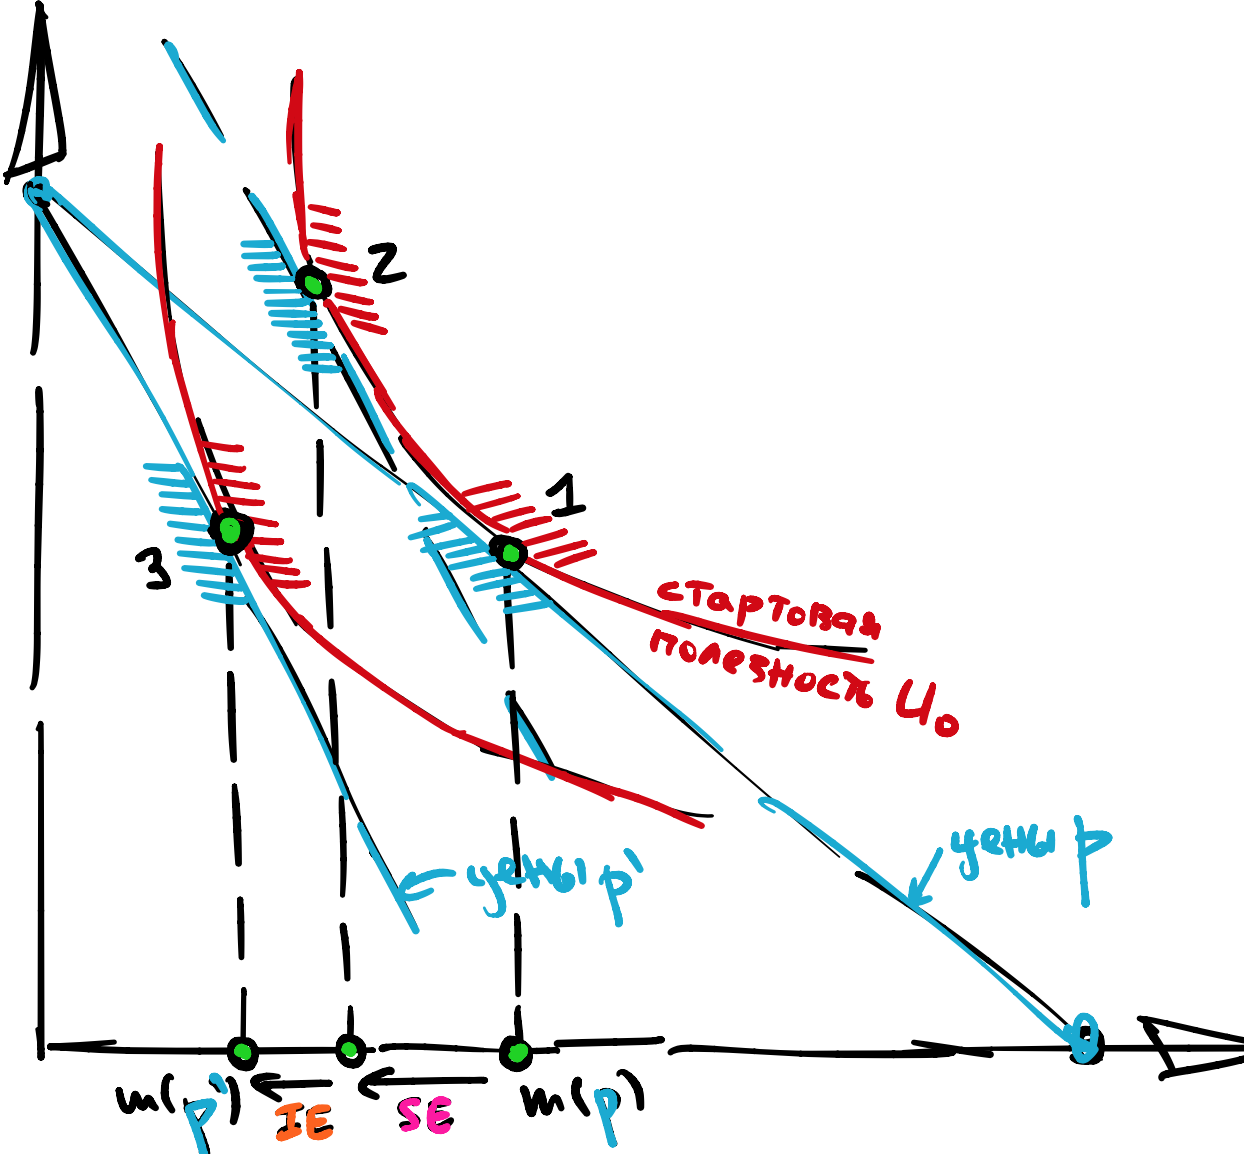
\includegraphics[width=.8 \textwidth]{SEIETE.png}
%\end{figure}
%
%\end{frame}
%
%\begin{frame}{Общий эффект}
%
%Есть также общий эффект (TE), он равен сумме эффекта замещения и эффекта дохода и представляет собой просто стандартное изменение маршаллианских спросов:
%
%$$ \text{TE} = \text{SE} + \text{IE} = m(p') - m(p).$$
%
%Поскольку маршаллианский спрос, как правило, наблюдаем, то можно считать, что общий эффект всегда известен. Неизвестно его разложение на эффект дохода и замещения.
%
%\end{frame}
%
%\section{Эффект замещения}
%
%\begin{frame}{Эффект замещения}
%
%Эффект замещения есть, по сути, приращение хиксианского спроса при полезности зафиксированной на изначальном уровне. 
%$$ SE = h(p', \bar U_0) - h(p, \bar U_0) $$
%
%Эффект замещения всегда отрицательный (неположительный, если быть точным), если он по своей цене, потому что мы доказали, что $\nabla^2 E \leqslant 0$.
%
%\end{frame}
%
%\begin{frame}{Эффект замещения}
%
%\begin{figure}[hbt]
%\centering
%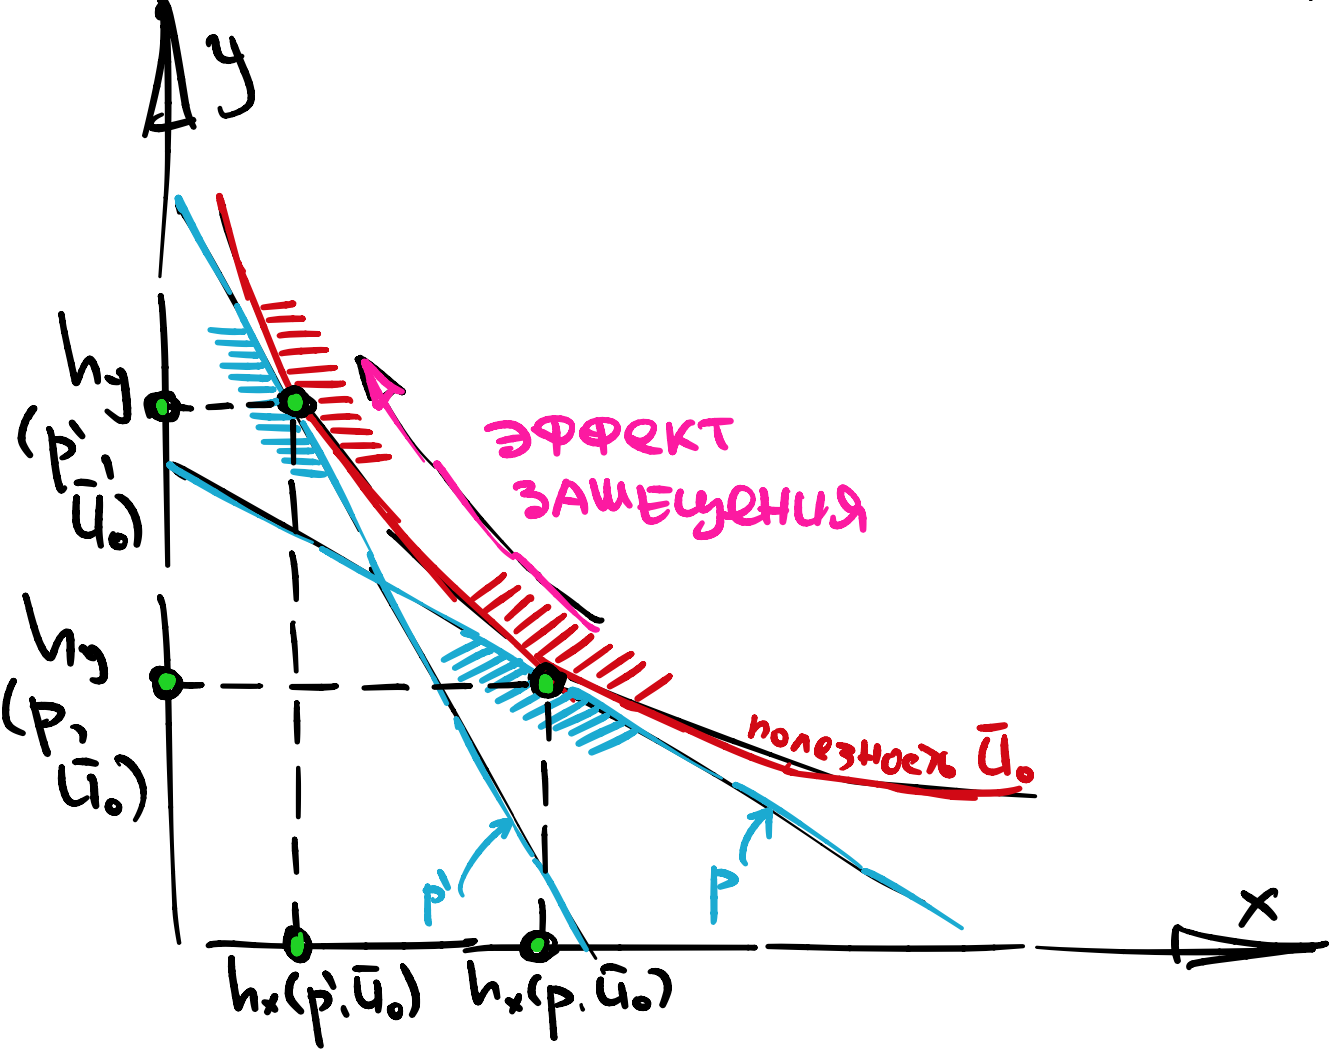
\includegraphics[width=.8 \textwidth]{SE.png}
%\end{figure}
%
%\end{frame}
%
%\section{Эффект дохода}
%
%\begin{frame}{Эффект дохода}
%
%Эффект дохода есть разница между общим эффектом и эффектом замещения, именно так его надо считать. 
%
%Однако сам по себе он не представляет большого интереса. Вообще не очень понятно, зачем вычислять кусок спроса, за который отвечает эффект дохода. 
%
%Гораздо интереснее понять, какому изменению бюджета соответствует эффект дохода? Тогда при любом изменении цен, мы можем сказать насколько мы "ограбили" того или иного потребителя в рублях.
%
%Это же как раз компенсирующая вариация $CV$!
%
%\end{frame}
%
%\begin{frame}{Эффект дохода}
%
%\begin{figure}[hbt]
%\centering
%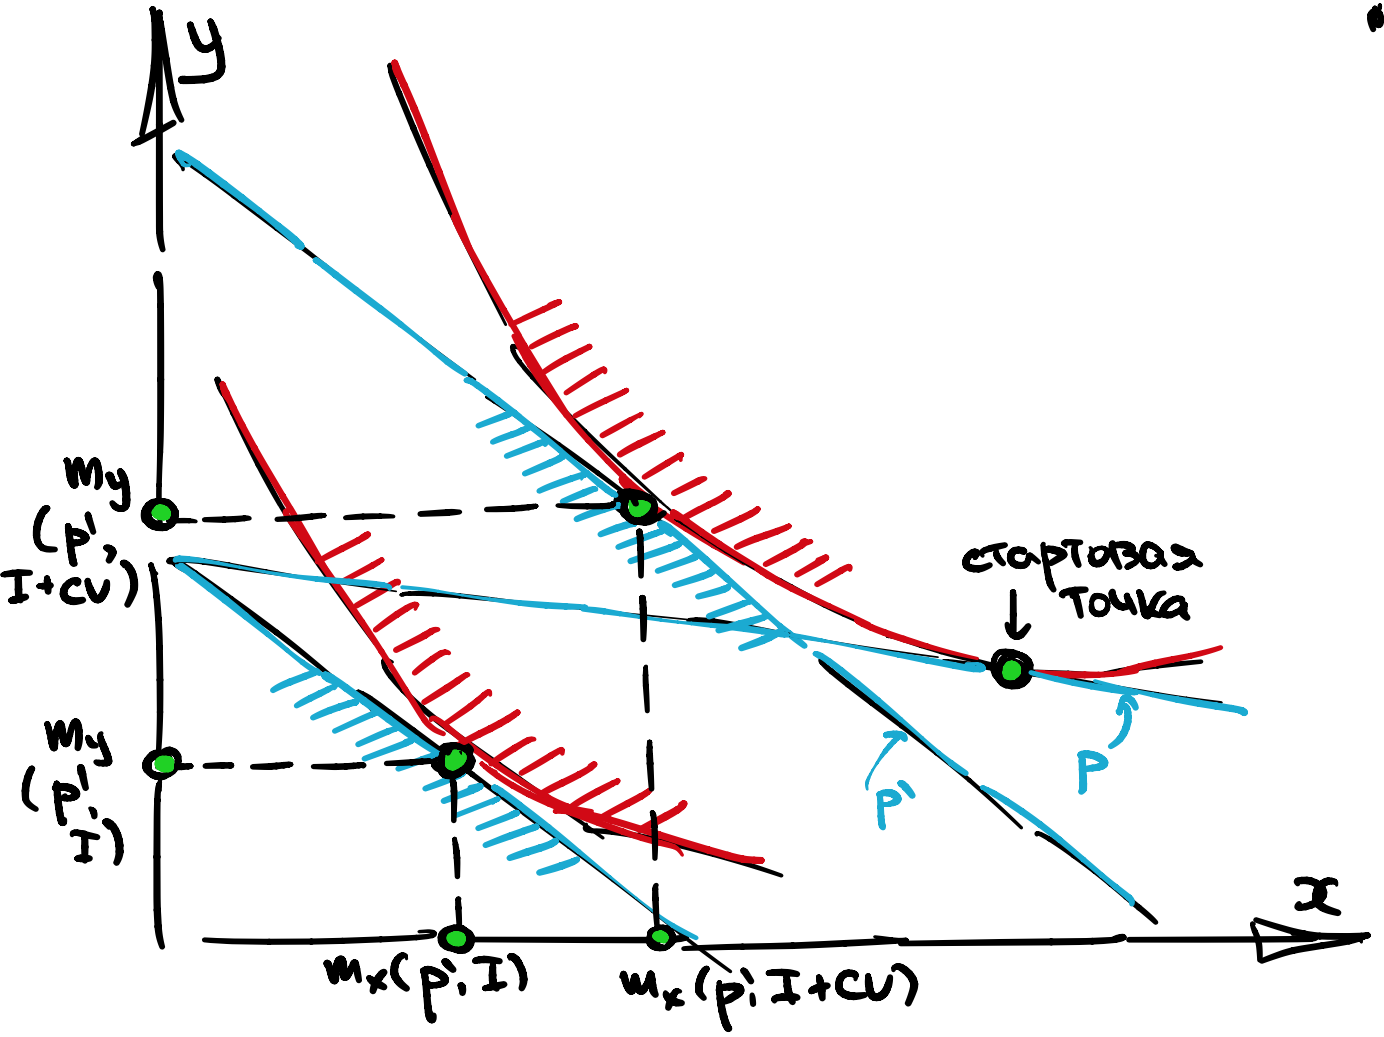
\includegraphics[width=.8 \textwidth]{IE.png}
%\end{figure}
%
%\end{frame}
%
%\section{Матрица Слуцкого}
%
%\begin{frame}{Матрица Слуцкого}
%
%Сфокусируемся на уравнении, связывающем Хиксианский и Маршаллианский спросы:
%$$\vec h (\vec p, \bar U) = \vec m(\vec p,  E(\vec p, \bar U)).$$
%Вас, скорее всего, не учили матричному дифференцированию, но в данном случае оно работает примерно как обычное:
%$$ \nabla \vec h(\vec p,  \bar U) = \nabla \vec m(\vec p,  \bar U) + \frac{\partial m}{\partial I} \cdot \nabla E(\vec p, \bar U) = \nabla \vec m(\vec p,  \bar U) + \frac{\partial m}{\partial I} \cdot \vec h $$
%Проблема в том, что и $\frac{\partial m}{\partial I}$ и $\vec h$ – это вектора длины $n$, и, поэтому, мы должны подумать, в каком порядке мы их хотим перемножить. 
%
%\end{frame}
%
%\begin{frame}{Матрица Слуцкого}
%
%$$ \nabla \vec h(\vec p,  \bar U) = \nabla \vec m(\vec p,  \bar U) + \frac{\partial m}{\partial I} \cdot \vec h $$
%
%Есть два варианта: либо мы умножаем строку $\frac{\partial m}{\partial I}$ на столбец $\vec h$, либо мы умножаем столбец $\frac{\partial m}{\partial I}$ на строку $\vec h$. 
%
%Один из этих вариантов даст число, а другой – матрицу. Тот вариант, который сохранит размерность объекта, и будет правильным матричным дифференцированием. 
%
%\end{frame}
%
%\begin{frame}{Матрица Слуцкого}
%
%В зависимости от того, что идет по строкам: координаты цен или координаты товаров – формула будет выглядеть по-разному. 
%
%Например, если по горизонтали идут товары, то правильно:
%$$ 
%(\nabla h_x, \nabla h_y) = (\nabla m_x, \nabla m_y) + 
%\begin{pmatrix} 
%h_x \\
%h_y
%\end{pmatrix} 
%\cdot (\frac{\partial m_x}{\partial I}, \frac{\partial m_y}{\partial I})
%$$
%
%Это называется \alert{уравнением Слуцкого}.
%
%Чтобы не запутаться, достаточно запомнить, что вектор $h$ в правой части уравнения – это, на самом деле $\nabla_{\vec p} E$, то есть он относится к ценам, которые идут по вертикали.
%
%\end{frame}
%\section{Зачем нужны матрицы Слуцкого}
%
%\begin{frame}{Матрица Слуцкого}
%Во-первых, матрица Слуцкого – это в некотором смысле четвертая модель поведения потребителя. То есть вместо калибровки полезности или предпочтений, мы можем калибровать матрицу замещения. 
%
%Коэффициенты матрицы Слуцкого можно переписать в терминах эластичности, дохода и долей, каждый из которых достаточно легко оценивается в данных. 
%\end{frame}
%
%\begin{frame}{Матрица Слуцкого}
%
%К примеру, если $s_x$ и $s_y$ это доли товаров $x, y$ в бюджете, то верхний диагональный элемент уравнения Слуцкого можно записать как:
%$$ \frac{\partial h_x}{\partial p} = \frac{m_x}{p} (\varepsilon_{x,p} + \varepsilon_{x,I} \cdot s_x)$$
%
%А диагональный элемент уравнения Слуцкого можно записать как:
%$$ \frac{\partial h_x}{\partial q} = \frac{m_x}{q} (\varepsilon_{x,q} + \varepsilon_{x,I} \cdot s_y)$$
%
%К слову, эти уравнения связывают эластичности хиксианского и маршаллианских спросов.
%
%\end{frame}
%
%\section{SE в первом приближении}
%
%\begin{frame}{SE в первом приближении}
%
%Матрица Слуцкого $S$ (она же $\nabla h=\nabla^2 E$) указывает нам на приращение Хиксианского спроса. 
%
%$$ SE = h(p') - h(p) = \int_p^{p'} \frac{\partial}{\partial p} h(x) dx \approx (p'-p) \nabla h = \delta p \cdot \nabla^2 E$$
%
%То есть если матрица оценена хорошо, то можно сказать, что приращение Хиксианского спроса – это приблизительно произведение матрицы Слуцкого на приращение цен. 
%
%А приращение Хиксианского спроса – это и есть $SE$.
%
%\end{frame}
%
%\section{Парадокс Гиффена}
%
%\begin{frame}
%
%Парадокс Гиффена заключается в том, что для некоторых товаров, которые пользовались популярностью у бедных: картофель и дешевый хлеб – наблюдалась прямая зависимость между ценой и спросом. Похожая зависимость иногда прослеживается для спроса на рис в современном Китае.
%
%Разрешение парадокса осуществляется за счет анализа Хиксианского спроса и матриц Слуцкого. 
%
%\end{frame}
%
%\begin{frame}
%
%Обратим внимание еще раз на эластичность Хиксианского спроса по собственной цене, которую я назову $\varepsilon^c_{x,p}$:
%$$\varepsilon^c_{x,p} = \varepsilon_{x,p} + \varepsilon_{x,I} \cdot s_{x},$$
%
%и перепишем ее так, чтобы маршаллианский спрос был слева:
%$$\varepsilon_{x,p} = \varepsilon^c_{x,p} - \varepsilon_{x,I} \cdot s_{x}.$$
%
%Легко видеть, что если $\varepsilon_{x,I} > 0$, то, поскольку $\varepsilon^c_{x,p}$ всегда неположительный, и $\varepsilon_{x,p}$ будет неположительный. А нам нужна положительная зависимость между $x,p$. 
%\end{frame}
%
%\begin{frame}
%
%Соответственно, можно сделать следующий вывод:
%
%\textbf{Нормальный товар не объяснит парадокс Гиффена.}
%
%\end{frame}
%
%\begin{frame}
%Предположим, наоборот, что товар $x$ инфериорный, то есть это товар низкого качества, тогда $\varepsilon_{x,I} < 0$. Предположим также, что доля товара $x$ в бюджете потребителя достаточно высока, то есть $s_{x}$ большой. Наконец, предположим, что для товара $x$ нет близкого (чистого) субститута, то есть $\varepsilon^c_{x,p}$ близок к нулю.
%
%Тогда может так случиться, что $\varepsilon_{x,p}$ станет положительным.
%
%\end{frame}
%
%\begin{frame}
%Еще раз
%$$\varepsilon_{x,p} = \varepsilon^c_{x,p} - \varepsilon_{x,I} \cdot s_{x}.$$
%
%\begin{itemize}
%\item $\varepsilon^c_{x,p}$ называется эффектом замещения
%\item $\varepsilon_{x,I} \cdot s_{x}$ называется эффектом дохода
%\end{itemize}
%
%Для того, чтобы объяснить парадокс Гиффена, нужно иметь слабый эффект замещения и сильный отрицательный эффект дохода.
%
%\end{frame}
%
%\begin{frame}
%\begin{figure}[hbt]
%\centering
%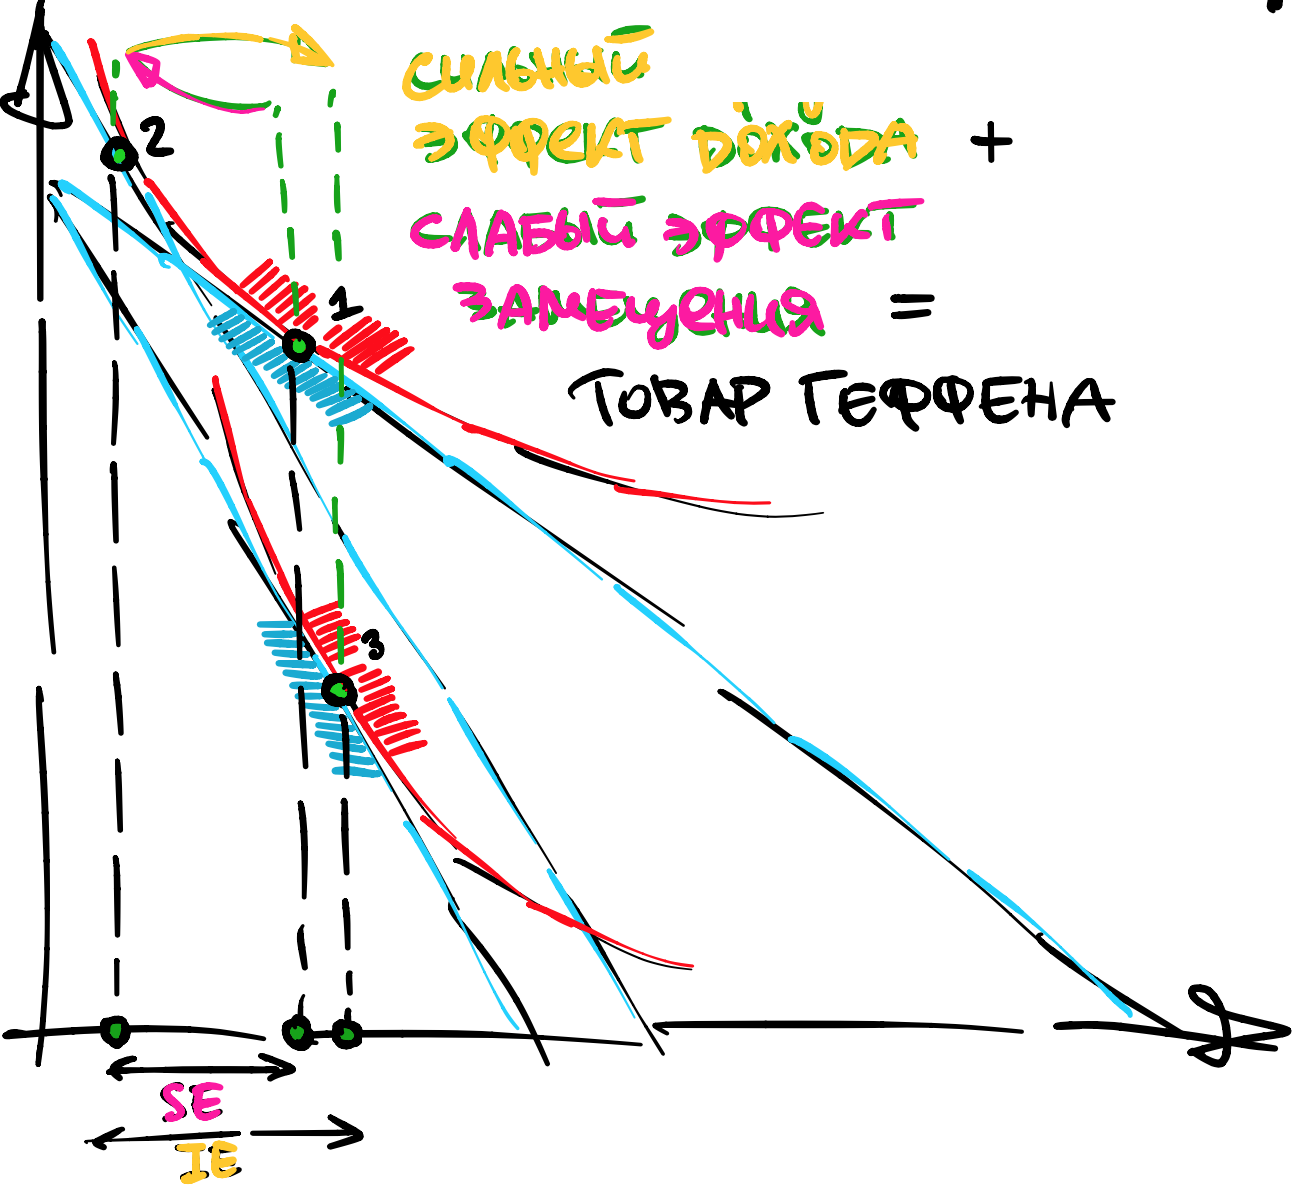
\includegraphics[width=.8 \textwidth]{IESE_CV.png}
%\end{figure}
%
%\end{frame}
%
%\section{Это была самая сложная лекция}

\end{document}